\documentclass{article}
\usepackage[utf8]{inputenc}
\usepackage[ukrainian]{babel}
\usepackage{graphicx}
\usepackage{hyperref}
\usepackage{tabularx}
\usepackage{booktabs}
\usepackage{xcolor}
\usepackage{subcaption}
\usepackage{float}
\usepackage[T2A]{fontenc}
\usepackage{amsmath}

\title{Модель пухлини на основі клітинного автомата}
\date{}

\begin{document}

\maketitle

\tableofcontents

\newpage

\section{Вступ}
Ракові захворювання є досить великою проблемо в сучасному світі, і нажаль ця проблема лише набирає обертів. Для кращого вивчення розвитку раку існують математичні моделі. Цей проєкт є однією з них, а точніше це симуляція що базується на клітинному автоматі.

\section{Теоретичні основи}
\subsection{Клітинні автомати в моделюванні раку}
Клітинний автомат базується на дискретному полі NxN, що при досить великиз значеннях надає досить точні та реалістичні результати. Клітинні автомати використовують стокастичний метод ітерування, тобто на кожному кроці дію клітини визначає якась випадкова подія. На клітину може впливати її оточення, наприклад концентрація ракових клітин. В цій симуляції на клітину впливають лише 8 сусідів розташованих у квадраті 3х3 з центром у даній.

\subsection{Ієрархія клітин пухлини}
Типи клітин використаних у симуляції:
\begin{itemize}
    \item Істинні стовбурові клітини (TSC) - клітини що не вмирають, можуть народжувати як собі подібних, так і і звичайні стовбурові клітини.
    \item Стовбурові пухлинні клітини (STC) - можуть лише звичайні ракові пухлини
    \item Звичайні пухлинні клітини (RTC) - пухлини, що породжують собіподібних, проте мають обмежену кількість поділів.
    \item Некротичні клітини - мертві клітини.
    \item Імунні клітини - клітини, що вюивають рак або вповільнюють його поділ.
\end{itemize}

\subsection{Динаміка росту пухлини}
Основні події життєвого циклу клітин:
\begin{itemize}
    \item Поділ - з деякою ймовірністю, за умови що клітина все ще може, вона створює нову клітину біля себе.
    \item Міграція - якщо клітина не поділяється, то є ймовірність, що вона переміститься в сусідню клітинку.
    \item Смерть - якщо у клітини закінчивсяс подільний потінціал або її знищила іммунна клітина, то вона помирає.
    \item Спокій - якщо жодна з вище перелічених подій не сталася, то клітина нічого не робить.
\end{itemize}

\subsection{Взаємодія з імунною системою}
Механізми імунної відповіді:
\begin{itemize}
    \item Активація - початок життя клітини, якщо вона була штучно внесена (наприклад нова доза препарату)
    \item Знищення клітин пухлини - якщо поруч знаходиться ракова клітина, то є шанс її знищити.
    \item Міграція та поділ імунних клітин - ідентично до поділу та міграції ракової пухлни описаних вище
    \item Тривалість життя імунних клітин - як і ракові клітини, імунні мають період життя, після якого помирають.
\end{itemize}

\section{Реалізація}
\subsection{Архітектура моделі}

Програмна архітектура моделі реалізована в об'єктно-орієнтованому стилі на мові Python. Основні компоненти:

\begin{itemize}
  \item \textbf{Решітка (\texttt{Grid})} --- клас, що представляє двовимірне середовище, у якому розташовані клітини. Кожна комірка решітки може містити одну клітину або бути порожньою. Забезпечує операції додавання, видалення та переміщення клітин, а також пошук сусідів.

  \item \textbf{Клас клітин (\texttt{Cell})} --- базовий клас для всіх типів клітин. Містить атрибути:
  \begin{itemize}
    \item тип клітини (стовбурова, диференційована, імунна),
    \item лічильники часу до поділу або смерті,
    \item ідентифікатор та координати у сітці.
  \end{itemize}
  Також реалізує методи поведінки: \texttt{divide()}, \texttt{migrate()}, \texttt{die()}.

  \item \textbf{Симулятор (\texttt{TumorSimulation})} --- головний клас, що відповідає за запуск симуляції. Містить об'єкти \texttt{Grid} і списки активних клітин. Керує всіма етапами симуляції: ініціалізацією, оновленням стану клітин, збором статистики та збереженням результатів.
\end{itemize}

Завдяки такій архітектурі модель є модульною, легко розширюється додаванням нових типів клітин або правил взаємодії.

\subsection{Основні параметри}

Налаштування симуляції визначаються в конфігураційному блоці або передаються через параметри командного рядка. Нижче описано ключові параметри моделі:

\begin{itemize}
  \item \textbf{Розміри сітки} (\texttt{grid\_size}) --- визначають кількість рядків і стовпців, тобто загальний розмір моделюваного середовища.
  \item \textbf{Початкова кількість клітин} --- кількість клітин кожного типу, які розміщуються у центрі сітки на початку симуляції.
  \item \textbf{Інтервал поділу клітини} (\texttt{division\_time}) --- число кроків симуляції, через які клітина може ділитись.
  \item \textbf{Ймовірність міграції} (\texttt{migration\_probability}) --- імовірність того, що клітина змінить свою позицію у сітці.
  \item \textbf{Імовірність смерті} (\texttt{death\_probability}) --- базова ймовірність апоптозу для кожного типу клітин.
  \item \textbf{Імунна відповідь} --- за бажанням можна активувати модуль імунної системи, що включає параметри швидкості руху імунних клітин та їх здатності знищувати пухлинні клітини.
  \item \textbf{Кількість кроків симуляції} (\texttt{n\_steps}) --- визначає загальну тривалість експерименту.
  \item \textbf{Насіння генератора випадкових чисел} (\texttt{random\_seed}) --- забезпечує відтворюваність результатів.
\end{itemize}

Параметри обираються таким чином, щоб наблизити модель до реалістичних біологічних процесів, але також допускають варіації для експериментів з різними сценаріями.

\subsection{Алгоритм симуляції}

Симуляція відбувається у дискретних часових кроках. На кожному кроці модель послідовно оновлює стан системи відповідно до таких етапів:

\begin{enumerate}
  \item \textbf{Оновлення клітин пухлини.}

  Для кожної клітини $i$ виконується стохастична оцінка подій. Ймовірність поділу клітини моделюється як:
\[
P_\text{divide}^{(i)} =
\begin{cases}
  p_\text{base}, & \text{якщо пройшов час до поділу і є вільне місце} \\
  0, & \text{інакше}
\end{cases}
\]

  Аналогічно, ймовірність смерті клітини (апоптозу) визначається як:
  \[
    P_\text{death}^{(i)} = p_\text{death}^{(t)} + \gamma \cdot n_\text{neighbors}^{(immune)}
  \]
  де $p_\text{death}^{(t)}$ --- базова ймовірність смерті для типу $t$, а $\gamma$ --- коефіцієнт впливу імунних клітин поблизу.

  Міграція відбувається з ймовірністю $P_\text{migrate}$ у випадковому напрямку на вільну сусідню позицію:
  \[
    P_\text{migrate}^{(i)} = p_\text{migrate} \cdot f(\text{density})
  \]
  де $f(\text{density})$ --- функція, що враховує щільність навколишнього середовища.

  \item \textbf{Оновлення імунних клітин (за потреби).}

  Імунна клітина переміщується за градієнтом концентрації пухлинних клітин $c(x,y)$:
  \[
    \vec{v}_\text{immune} = -\nabla c(x, y)
  \]
  Якщо вона потрапляє на клітину пухлини, вона може її знищити з ймовірністю $P_\text{kill}$.

  \item \textbf{Збір статистики.}

  Після кожного кроку підраховуються наступні характеристики:
  \[
    N_t^{(k)} = \text{Кількість клітин типу } k \text{ на кроці } t
  \]
  \[
    A_t = \sum_{i=1}^N \mathbb{1}_{\text{alive}}(i)
  \]
  де $\mathbb{1}_{\text{alive}}(i)$ --- індикатор, що клітина $i$ жива.
\end{enumerate}

Таким чином, симуляція імітує складну динаміку пухлини, враховуючи стохастичність процесів та просторові взаємодії клітин.
\section{Результати симуляції}

\subsection{Візуалізація та колірна схема}

Для інтерпретації результатів симуляції застосовується наступна колірна схема клітин:

\begin{itemize}
    \item \textcolor{blue}{\rule{1em}{1em}} Імунні клітини (Immune cells)
    \item \textcolor{orange}{\rule{1em}{1em}} Некротичні клітини (Necrotic cells)
    \item \textcolor{gray}{\rule{1em}{1em}} Порожні клітини (вільний простір)
    \item \textcolor{yellow}{\rule{1em}{1em}} Істинні стовбурові клітини (True Stem Cells)
    \item \textcolor{green}{\rule{1em}{1em}} Стовбурові пухлинні клітини (Stem Tumor Cells)
    \item \textcolor{red}{\rule{1em}{1em}} Звичайні пухлинні клітини (Regular Tumor Cells), з градацією відтінків залежно від кількості поділів
\end{itemize}

\subsection{Динаміка росту пухлини без імунної відповіді}
На рисунках нижче показано просторову динаміку росту пухлини без впливу імунної системи. Видно поступове збільшення маси пухлини та утворення некротичного ядра.

\begin{figure}[H]
    \centering
    \begin{subfigure}[t]{0.32\linewidth}
        \centering
        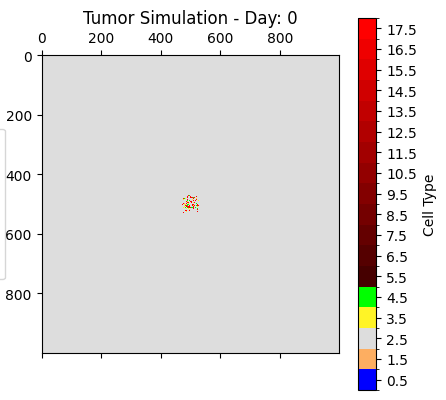
\includegraphics[width=\linewidth]{tumor_simulation_stats/tumor_day_0.png}
        \caption{День 0}
        \label{fig:tumor-day-0-no-immune}
    \end{subfigure}
    \hfill
    \begin{subfigure}[t]{0.32\linewidth}
        \centering
        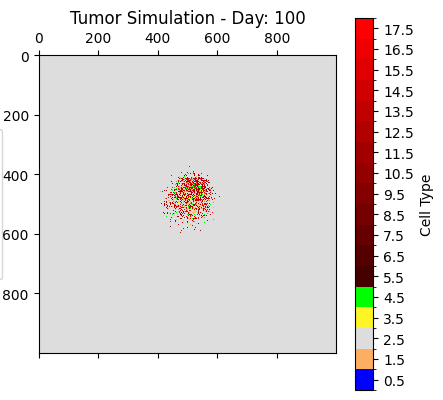
\includegraphics[width=\linewidth]{tumor_simulation_stats/tumor_day_100.png}
        \caption{День 100}
        \label{fig:tumor-day-100-no-immune}
    \end{subfigure}
    \hfill
    \begin{subfigure}[t]{0.32\linewidth}
        \centering
        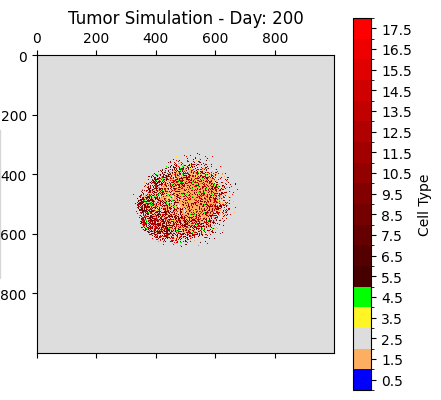
\includegraphics[width=\linewidth]{tumor_simulation_stats/tumor_day_200.png}
        \caption{День 200}
        \label{fig:tumor-day-200-no-immune}
    \end{subfigure}
    \label{fig:tumor-evolution-no-immune}
\end{figure}

\subsection{Динаміка росту пухлини з імунною відповіддю}
Далі представлено вплив імунної системи на динаміку пухлини. Імунні клітини поступово проникають у пухлину, взаємодіють з нею, зменшуючи кількість активних пухлинних клітин.

\begin{figure}[H]
    \centering
    \begin{subfigure}[t]{0.32\linewidth}
        \centering
        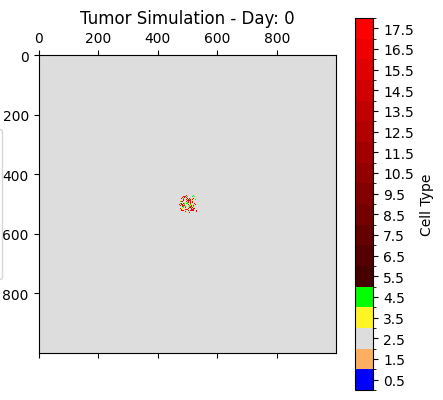
\includegraphics[width=\linewidth]{tumor_immune_simulation_stats/tumor_immune_day_0.png}
        \caption{День 0}
        \label{fig:tumor-day-0-immune}
    \end{subfigure}
    \hfill
    \begin{subfigure}[t]{0.32\linewidth}
        \centering
        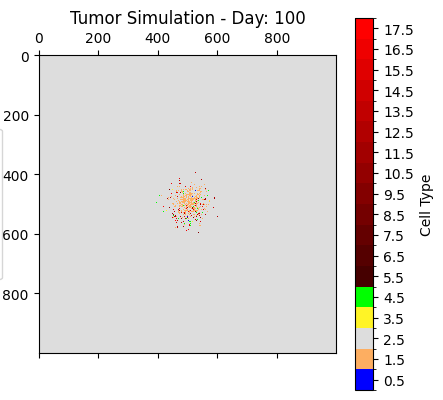
\includegraphics[width=\linewidth]{tumor_immune_simulation_stats/tumor_immune_day_100.png}
        \caption{День 100}
        \label{fig:tumor-day-100-immune}
    \end{subfigure}
    \hfill
    \begin{subfigure}[t]{0.32\linewidth}
        \centering
        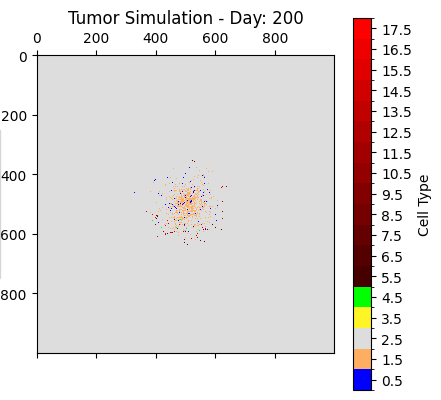
\includegraphics[width=\linewidth]{tumor_immune_simulation_stats/tumor_immune_day_200.png}
        \caption{День 200}
        \label{fig:tumor-day-200-immune}
    \end{subfigure}
    \label{fig:tumor-evolution-immune}
\end{figure}

\subsection{Графіки популяцій клітин}
На графіках показано кількісні зміни популяцій клітин протягом симуляції. Це дозволяє оцінити темпи росту пухлини, активність імунної системи, а також частку некротичних клітин.

\begin{figure}[H]
    \centering
    \begin{subfigure}[t]{0.75\linewidth}
        \centering
        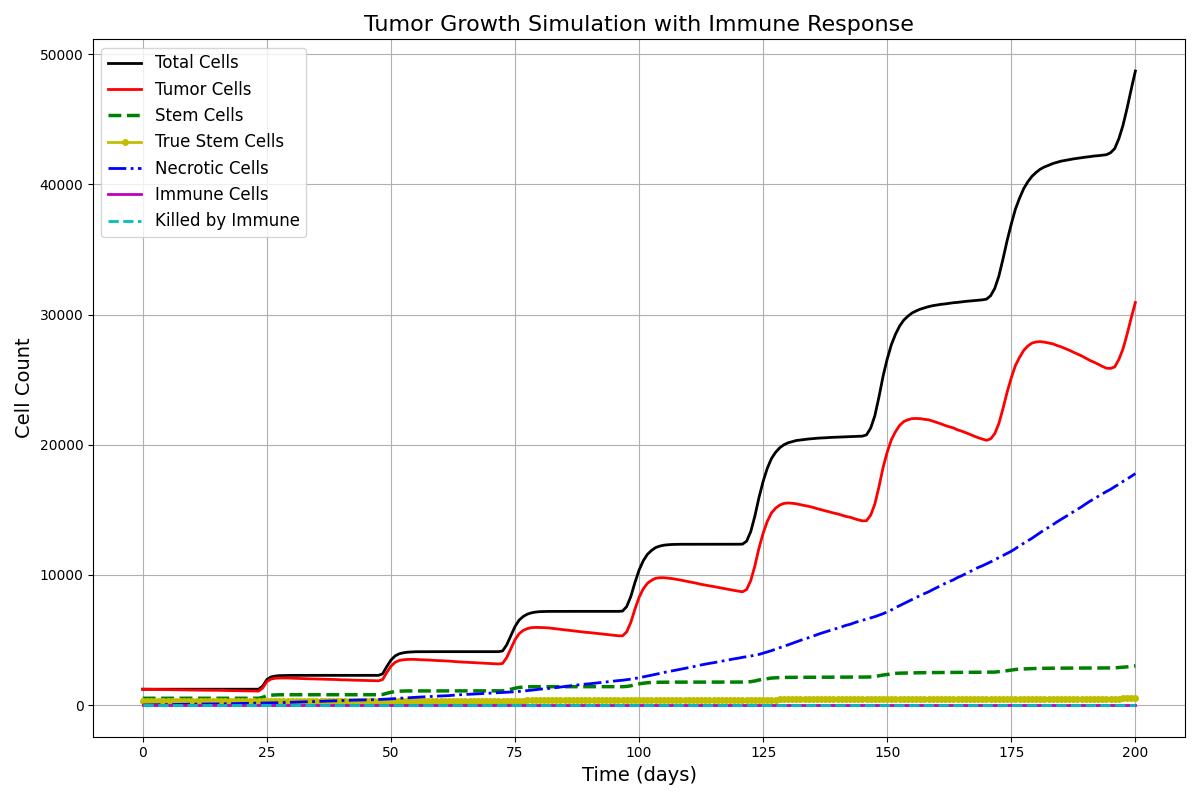
\includegraphics[width=\linewidth]{tumor_simulation_stats/tumor_stats.png}
        \caption{Динаміка популяцій клітин без імунної відповіді}
        \label{fig:tumor-stats-no-immune}
    \end{subfigure}

    \begin{subfigure}[t]{0.75\linewidth}
        \centering
        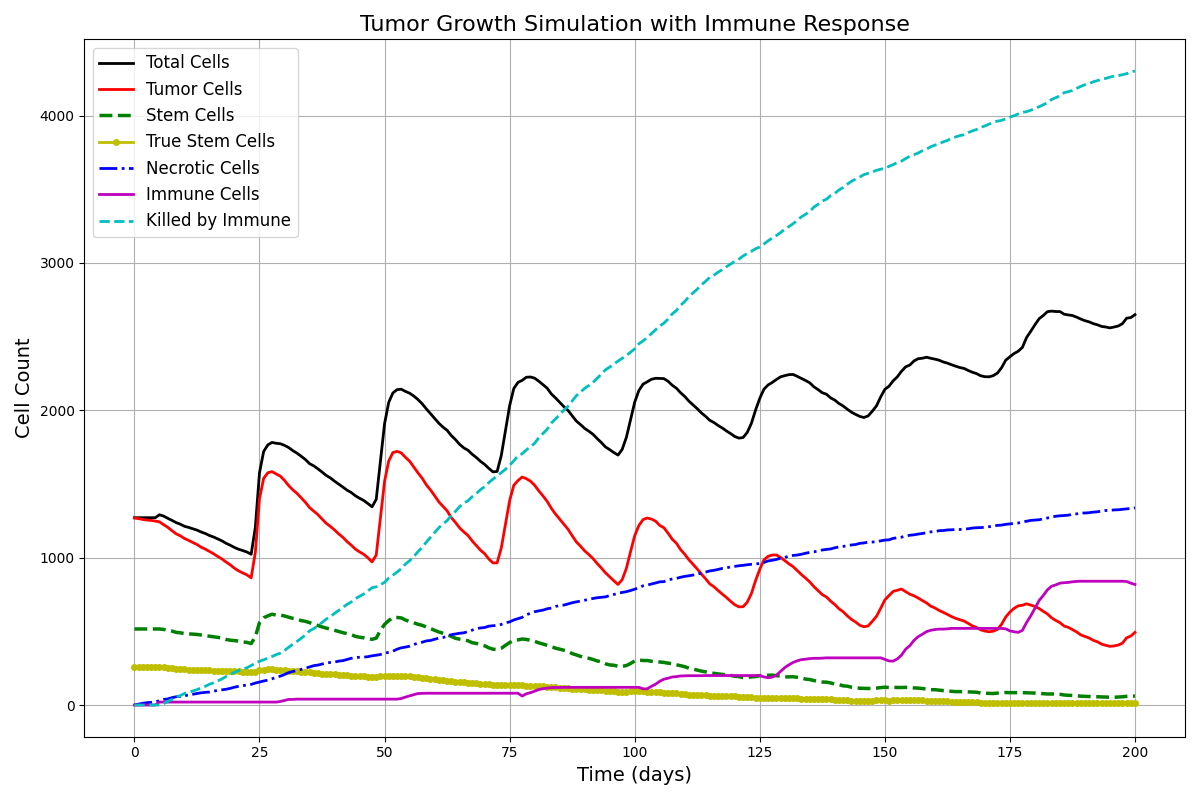
\includegraphics[width=\linewidth]{tumor_immune_simulation_stats/tumor_immune_stats.png}
        \caption{Динаміка популяцій клітин з імунною відповіддю}
        \label{fig:tumor-stats-immune}
    \end{subfigure}
    \label{fig:stats-comparison}
\end{figure}

\section{Учасники проєкту}
\begin{itemize}
    \item Ярина Печененко – логіка клітин
    \item Іван Зарицький – візуалізація, CLI
    \item Михайло Рихальський – структура решітки, просторова логіка
    \item Роман Прохоров – движок симуляції
\end{itemize}

\section{Ментор}
Максим Жук
\begin{thebibliography}{99}

\bibitem{david2022}
Sergio A. David, Carlos A. Valentim, José A. Rabi. \textit{Cellular-automaton model for tumor growth dynamics: Virtualization of different scenarios}.\\
\href{https://www.sciencedirect.com/science/article/pii/S0010482522011891}{https://www.sciencedirect.com/science/article/pii/S0010482522011891}

\bibitem{sabzpoushan2019}
S. H. Sabzpoushan. \textit{A cellular automata model of chemotherapy effects on tumour growth: targeting cancer and immune cells}.\\
\href{https://www.tandfonline.com/doi/full/10.1080/13873954.2019.1571515}{https://www.tandfonline.com/doi/full/10.1080/13873954.2019.1571515}

\end{thebibliography}

\end{document}